\documentclass[a4paper, 12pt]{article}
\usepackage[slovene]{babel}
\usepackage[utf8]{inputenc}
\usepackage[T1]{fontenc}
\usepackage{lmodern}
\usepackage{amsmath, amsfonts}
\usepackage{graphicx}

%\graphicspath{ {C:\Users\Lenovo\Desktop\FMF\Magisterij\Matematika z racunalnikom\Hungarian-method\slike} }

\newtheorem{definition}{Definition}

\title{Madžarska metoda - poročilo}
\author{Borut Zupan}
\date{24. 5. 2022}

\begin{document}
\maketitle

\section{Definicije}
Za razumevanje, kaj počne madžarska metoda si moramo najprej pogledati nekaj definicij.
\begin{definition}
    Poln dvodelen graf je graf, kjer vozlišča lahko razdelimo
    na dve disjunktni množici $U$ in $V$ tako, da je vsako vozlišče
    iz $U$ povezan z vsakim vozliščem iz $V$. Povezav med vozlišči iz $V$
    in med vozlišči iz $U$ ni.
\end{definition}

Sedaj, ko vemo s kakšnimi grafi delamo, si poglejmo kakšne podgrafe opazujemo.

\begin{definition}
    \begin{itemize}
        \item Množica $M$ povezav grafa $G$ je prirejanje v $G$, če povezave iz $M$ nimajo skupnih krajišč. 
        \item Množica $P$ vozlišč grafa $G$ je pokritje v $G$, če ima vsaka povezava grafa $G$ vsaj eno krajišče v $P$.
    \end{itemize}
\end{definition}

Madžarska metoda za dvodelne grafe ima utež. To, da je graf z utežmi pomeni, da obstaja funkcija,
ki priredi vsaki povezavi neko število.

Madžarska metoda za dvodelne grafe z utežmi poišče največjega prirejanja v dvodelnem grafu $G$.
Poleg največjega prirejanja v $G$ nam ta metoda poišče tudi najmanjše pokritje v $G$. Seveda, pa
ni težko prevesti problem na iskanje največjega pokritja v $G$.

\section{Madžarksa metoda za dvodelne grafe z utežmi}
Za madžarsko metodo rabiš naslednje vhodne podatke:
\begin{enumerate}
    \item Poln dvodelen graf $G$, kjer je $V(G) = X \cup Y$ dvodelna razdelitev, $X = \{x_1,\ldots,x_n\}$
            in $Y = \{y_1,\ldots,y_m\}$.
    \item Matrika cen povezav $C \in \mathbb{R}^{n\times m}$.
\end{enumerate}

Metoda ti vrne najcenejše popolno prirejanje v $G$, pri čemer je cena prirejanja $M \subseteq E(G)$ enaka
$$ c(M) = \sum_{x_iy_j \in M}c_{ij}. $$

Postopek ima več korakov. Ti so naslednji:
\begin{enumerate}
    \item Zarotiramo matriko cen povezav tako, da bo stolpcev vsaj toliko kot vrstic in 
            definiramo $k = \min{(n,m)}$. Pojdi na točko 2.
    \item Od elementov vsake vrstice matrike $C$ odštejemo najmanjši element vrstice. Pojdi
            na točko 3.
    \item V tej novi matriki najdi ničlo $N$. Označi jo z zvezdico, če v vrstici in stolpcu ničle
            N ni nobene druge ničle z zvezdico. To nadaljuj za vsak element matrike. Pojdi na točko 4.
    \item Pokrij vsak stolpec, ki vsebuje ničlo z zvezdico. Če je pokritih $k$ stolpcev, pojdi na 
            zadnjo točko. Drugače pojdi na točko 5.
    \item Najdi nepokrito ničlo in jo označi z črtico. Če ni nobene ničle z zvezdico v vrstici te
            ničle s črtico pojdi na točko 6. Drugače, pokrij vrstico z ničlo s črtico in razkrij
            stolpec, ki vsebuje ničlo z zvezdico. Nadaljuj ta postopek, dokler ni več nobene nepokrite
            ničle. Shrani najmanjšo nepokrito vrednost v matriki in pojdi na točko 7.
    \item Skonstruiraj zaporedje ničel s črtico in ničel z zvezdico na naslednji način. Naj bo $N_0$ ničla
            ničla s črtico iz točke 5. Z $N_1$ označimo ničlo z zvezdico, ki je v istem stolpcu kot $N_0$ (če obstaja).
            Z $N_2$ označi ničlo s črtico v isti vrstici kot $N_1$. Nadaljuj dokler se zaporedje ne ustavi
            na ničli s črtico, ki nima nobene ničle z zvedico v njenem stolpcu. V tem zaporedju vse ničle s
            črtico spremeni v ničle z zvedico in vse ničle z zvezdico odznači. Vsa pokritja odpokrij in pojdi
            na točko 4.
    \item Dodaj vrednost iz točke 5 vsakem elementu pokritih vrstic in odštej vrednost iz točke 5 vsakemu
            elementu nepokritih stolpcev. Pojdi nazaj na točko 5.
    \item Najcenejše popolno prirejanje predstavljajo indeski ničel z zvezdico.
\end{enumerate}

Metodo sem impelementrial v \textit{Pythonu} s pomočjo knjižnice \textit{numpy},
ker ima veliko vgrajenih funkcij za delo z matrikami.

Uporabniški vmesnik sem prav tako implementiral v \textit{Pythonu} s pomočjo
knjižnice \textit{tkinter}, ki omogoča enostavno in hitro gradnjo uporabniškega
vmesnika.

V uporabniškem vmesniku lahko skonstruiraš svojo matriko cen povezav in preveriš
kakšna je njeno najcenejše ali najdražje prirejanje. Metoda ti vrne tudi koliko
časa je algoritem porabil za izračun le tega.

Druga opcija pa je, da narediš eno ali več naključnih matrikk cen povezav in
pogledaš kakšno je njihovo povprečno najcenejše ali najdražje prirejanje in
kakšen je povprečen čas izvajanja metode na takih matrikah. Te rezultati si
bomo še malo bolj ogledali v naslednjem razdelku.

\section{Rezultati}

Torej imamo naključne matrike, kjer so elementi iz neke porazdelitve. Uporabili
bomo uniformno porazdelitev, zanimivo pa bi bilo rezultate pogeldati tudi še v
kakšni drugi porazdelitvi. Omejili se bomo na kvadratne matrike.

Najprej si poglejmo rezultate na malo manjšem primeru. Vzeli bomo $1000$ matrik
velikosti $10 \times 10$, ki imajo za elemente naključna števila med $1$ in vključno
z $9$. Računali bomo najcenejše prirejanje, torej prirejanje, ki ima najmanjšo ceno.

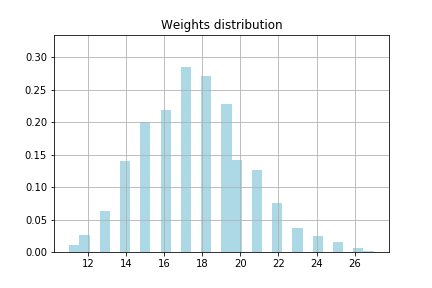
\includegraphics[width=\textwidth]{../slike/picture1011min.png}

Povprečen čas izvedbe algoritma je $0,002$ sekunde, maksimalen čas je $0,012$ sekunde, minimalen pa $0,00056$.

Opazimo, da porazdelitev izgleda kot normalna porazdelitev z povprečjem med $17$ in $18$.
Minimalna cena je $11$, maksimalna pa $27$. 

Čas izvedbe je majhen, kar je primerno, ker ima matrika majhno velikost. Razlika med maksimalnim
in minimalnim časom tudi ni velika.

\hfill \break
Poglejmo si še za primer, ko izračunamo najdražje prirejanje oz. lahko si to predstavljamo
kot maksimalen profit.

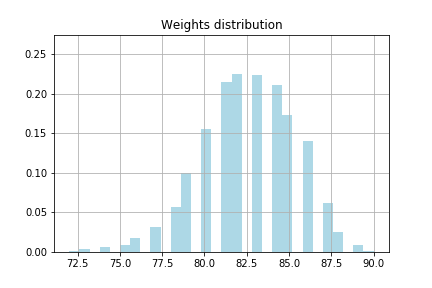
\includegraphics[width=\textwidth]{../slike/picture1011max.png}

Povprečen čas izvedbe algoritma je $0,002$ sekunde, maksimalen čas je $0,011$ sekunde, minimalen pa $0,00061$.

Povprečen profit je okrog $82,5$. Maksimalen profit je $90$, kar je tudi največ kar lahko
dobimo. Primer matrike s tako ceno oz. profitom je taka, ki ima na diagonale same $9$.
Najmanjši profit pa je $72$.

Povprečen čas izvedbe je enak kot če bi računali najcenejše prirejanje.
To ni presenetljivo, ker za izračun maksimalne
cene matriko transformiramo samo z odštevanjem profitne matrike od matrike enake velikost, kjer so 
vsi elementi maksimalen element profitne matrike. S tem dobiš matriko cen, za katero računaš
najcenejše prirejanje. Matriki imata enako velikost in imata
podobno strukturo, zato imata tudi zelo podobne čase.

\hfill \break
Povečajmo sedaj velikost matrike. Poženimo Madžarsko metodo tokrat na $100$ matrikah
velikosti $100 \times 100$. Obdržimo razpon števil med $1$ in $9$ in izračunajmo
ceno najcenejšega prirejanja.

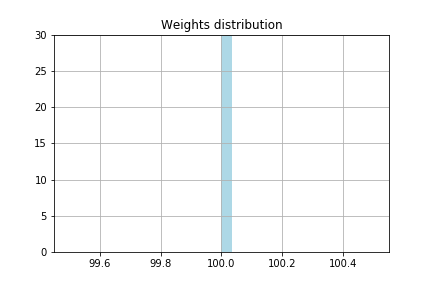
\includegraphics[width=\textwidth]{../slike/picture111min.png}

Povprečen čas izvedbe je $2,4$ sekunde, maksimalen čas je $3,5$ sekunde, minimalen pa $1,4$
sekunde.

Povprečen čas je znatno večji, ker smo imeli večjo matriko. Opazi se tudi velika razlika med
maksimalnim in minimalnim časom, kar pomeni, da je struktura matrike oz. porazdelitev 
števil v matriki pomembna za hitrost algoritma.

Opazimo, da je za vse matrike optimalna cena enaka. To se zgodi, ker imamo veliko 
matriko v primerjavi z razponom števil v matriki. Če bi imeli večji razpon števil,
se to ne bo zgodilo, kar pokažemo z naslednjim primerom:

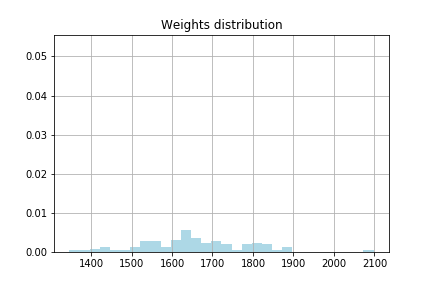
\includegraphics[width=\textwidth]{../slike/picture1101min.png}

Vzeli smo naključna števila med $1$ in $1000$.

\hfill \break
Poglejmo si še kako raste čas z večanjem velikosti matrike.

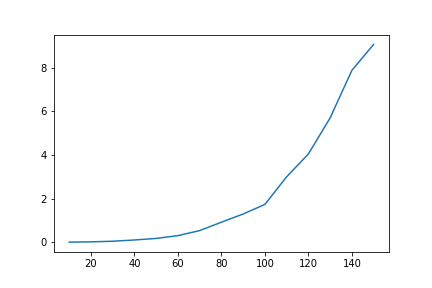
\includegraphics[width=\textwidth]{../slike/algorithm_time.png}

Na abcisni osi so velikosti matrik, na ordinatni osi pa čas v sekundah.
















\end{document}